本书旨在告诉您,如何快速高效地从互联网上获取信息,以及如何避免来自广告、垃圾内容、恶意软件的骚扰。

由于您阅览的文件可能并非最新版本------这意味着有些东西会在未来失效------因此您应该考虑访问本手册的网页版本:\url{https://yaii-project.github.io/}

\section{入门章节}\label{ux5165ux95e8ux7ae0ux8282}

\subsection{浏览器是您访问互联网的入口}\label{ux6d4fux89c8ux5668ux662fux60a8ux8bbfux95eeux4e92ux8054ux7f51ux7684ux5165ux53e3}

您的电脑桌面上可能有这样一个图标:
\includegraphics[width=0.69792in,height=0.92708in]{media/image1.png}

它(Internet
Explorer)是微软开发的一款网页浏览器,它很旧,即便是IE11也已经结束了它的生命周期(这意味着您永远都不会接收到关于它的更新了)。

为了访问现代网页,您需要一个有更新的浏览器。

您可以从\url{https://www.mozilla.org/firefox/all/\#product-desktop-esr}下载Firefox浏览器,打开网页后点击【立即下载】:

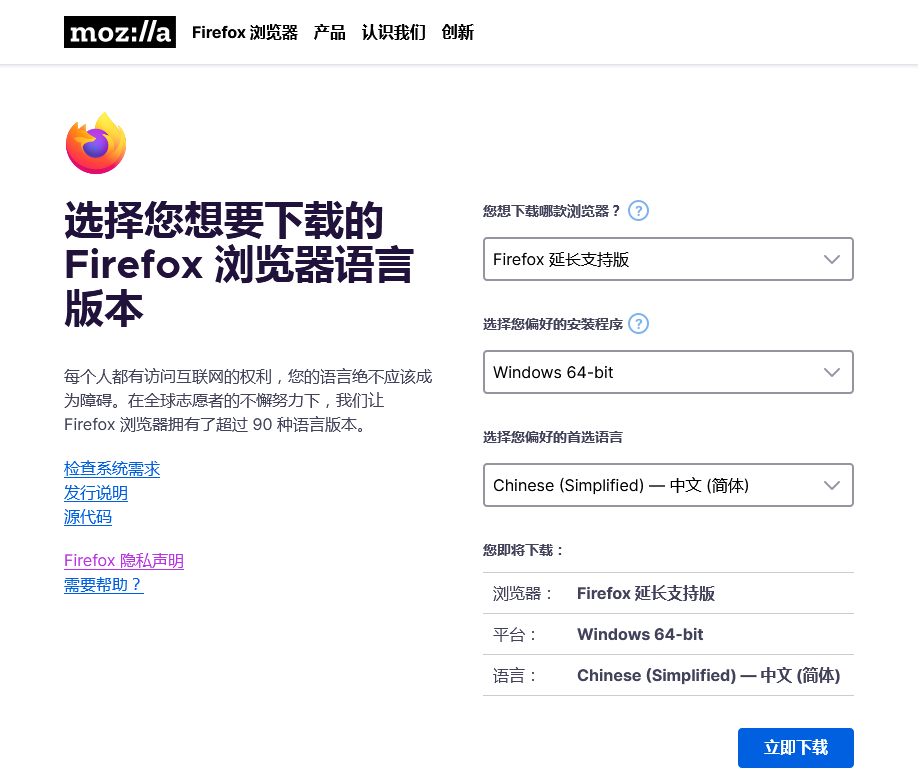
\includegraphics[width=3.64168in,height=3.0625in]{media/image2.png}

图中显示的选择是【Firefox延长支持版】,这是考虑到仍然有Windows
7/8/8.1用户在阅读本手册,如果您使用的是Windows
10/11等更新版本,请选择【Firefox】。

*注:Windows XP或更老版本请考虑升级,本手册无法为您提供任何建议。

*提示:有关如何辨认系统版本,请参阅本手册的【】章节。

*提示:Linux系统用户请参阅本手册的【】章节。

接下来的教程使用延长支持版作为示例,不同版本的浏览器在操作上存在些许差异,如果您发现有不同之处,请寻找有相近功能的按钮/入口。

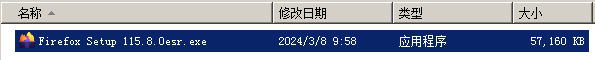
\includegraphics[width=5.76806in,height=0.58148in]{media/image3.png}

作为访问互联网的入口,浏览器可以为您提供大部分的功能,双击运行上图所示的安装程序以开始安装。

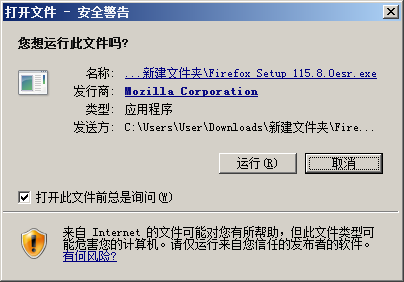
\includegraphics[width=2.68069in,height=1.87118in]{media/image4.png}这个界面是为了保护您的电脑不受病毒侵扰,特此向您确认是否要继续。请按【运行】。

接下来的安装界面如图所示:

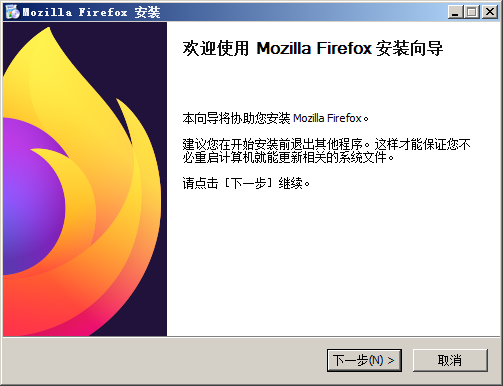
\includegraphics[width=2.57907in,height=1.97917in]{media/image5.png}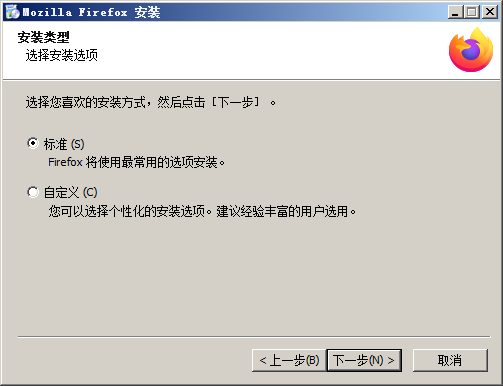
\includegraphics[width=2.57874in,height=1.97891in]{media/image6.png}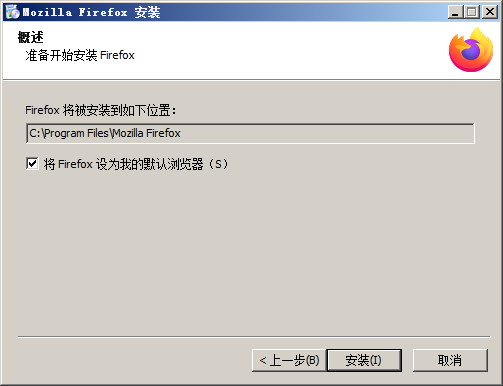
\includegraphics[width=2.57874in,height=1.97891in]{media/image7.png}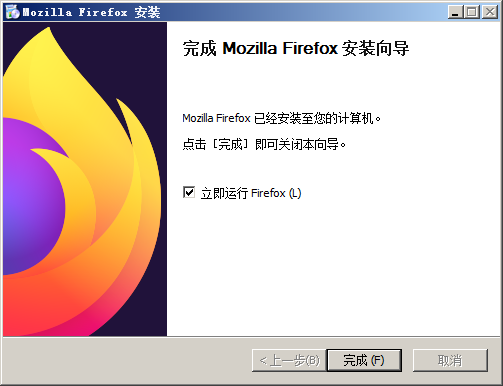
\includegraphics[width=2.57914in,height=1.97922in]{media/image8.png}

运行Firefox后您会看到此界面:

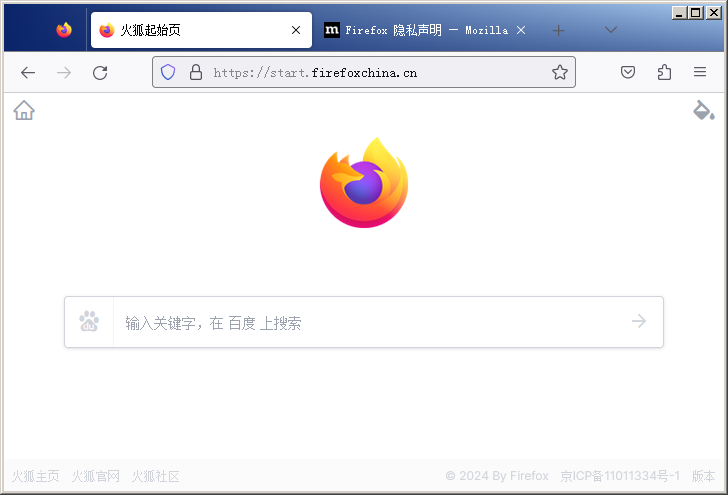
\includegraphics[width=5.76806in,height=3.92214in]{media/image9.png}
